\chapter{The Power of Small Toric Codes} 
\label{ch:SurfaceCodes}

\section{Introduction to the Toric Code}

The ability to correct and recover from errors is important for any quantum computing scheme. The discovery of the first error correcting quantum codes by Shor and Steane \cite{shor_codes_95, steane_code_96, steane_code_96_2} was vital for demonstrating that quantum computing was theoretically viable. The toric code is an error correcting code proposed by Kitaev \cite{kitaev_1, kitaev_2}, arising from work using quantum mechanics to provide simple models of topological order. It can be regarded as the simplest and most elegant in the class of such codes, collectively known as surface codes \cite{kitaev_bravyi, planar_codes_freedman_meyer}.

One of the key advantages of surface codes is their local nature - the codes can be implemented on a two-dimensional lattice of qubits using only nearest neighbour interactions. In this realistic experimental scenario, surface codes can tolerate per-operation error rates of up to 1\% \cite{fowler11, fowler_classical_processing}, compared with rates in of the order of $10^{-4}$ for the early error correcting codes \cite{steane_code_shit}.

In this chapter we look towards an experimental realisation of the toric code and study the code for small values of $n$. We pre-compute a decoding library, an approach that quickly becomes intractable for values of $n$ above those considered here, but has the advantage that we obtain a provably optimum decoding success rate. We use our pre-computed decoder to assess the \textit{encoding power} of the code: we say the code has positive encoding power if the encoded qubits exhibit a lower error rate than the same number of unencoded qubits subjected to the same noise.

\section{Shor's Code Revisited}

Before moving on to the toric code, we first look at a simple example of an error correcting code in order to introduce some of the notation and concepts that we use later. For this purpose we pick the first stage of Shor's code \cite{shor_codes_95}. The full code uses nine qubits to protect against general errors; the code we analyse here uses only three qubits and protects only against a single error channel. We describe the code by specifying how to encode a general qubit:
\begin{align}
  \alpha\ket{0} + \beta\ket{1} \rightarrow \alpha\ket{000} + \beta\ket{111}.\label{shor_state}
\end{align}
The idea here is very simple: each logical qubit is encoded into three physical qubits. Shor constructed a circuit such that if there was a bit-flip error - interchanging $\ket{0} \leftrightarrow \ket{1}$ -  on any one of the three qubits, the state would automatically be corrected. The system basically implements a `majority vote' error correction scheme.

We now develop a different description of the code, which will directly translate to our treatment of the toric code later in the chapter. In order to do this we first introduce the standard qubit operators:
\begin{align}
  Z &= \ket{0}\bra{0} - \ket{1}\bra{1} \\
  X &= \ket{0}\bra{1} + \ket{1}\bra{0} \\
  Y &= \ket{0}\bra{1} - \ket{1}\bra{0} = ZX.
\end{align}
In what follows we will need to apply these operators to states of multiple qubits. To do this we will introduce subscripts to the operators, so that, for example, $Z_1$ is the $Z$ operator acting on the first qubit. Operators acting on different qubits can be seen to commute with one another.

\begin{table}
  \begin{center}
    \begin{tabular}{c c c c c}
      State & $Z_1 Z_2$ & $Z_2 Z_3$ & $Z_1 Z_3$ & $Z_1$ \\
      \hline
      $\ket{000}$ & $+1$ & $+1$ & $+1$ & $+1$ \\
      $\ket{001}$ & $+1$ & $-1$ & $-1$ & $+1$ \\
      $\ket{010}$ & $-1$ & $-1$ & $+1$ & $+1$ \\
      $\ket{100}$ & $-1$ & $+1$ & $-1$ & $-1$ \\
      $\ket{110}$ & $+1$ & $-1$ & $-1$ & $-1$ \\
      $\ket{101}$ & $-1$ & $-1$ & $+1$ & $-1$ \\
      $\ket{011}$ & $-1$ & $+1$ & $-1$ & $+1$ \\
      $\ket{111}$ & $+1$ & $+1$ & $+1$ & $-1$
    \end{tabular}
  \end{center}
  \caption{The eigenvalues of the operators on their simultaneous eigenstates}
  \label{shor_states}
\end{table}

We will start by considering a state of three qubits and the set of operators $S = \{Z_1Z_2, Z_2Z_3, Z_1Z_3\}$. As these operators commute with one another it is possible to find states that are simultaneous eigenstates of all three. For the set $S$ that we have chosen, the simultaneous eignenstates can be taken to be the $Z$ basis vectors, as shown in Table~\ref{shor_states}. Note that the set of eigenvalues vary with the state, but the third column is the product of the first two. The operators we have chosen are not actually independent as
\begin{align}
  (Z_1Z_2)(Z_2Z_3) = Z_1Z_3.
\end{align}
To break the degeneracy in the eigenstates we introduce a fourth operator $Z_1$ that commutes with the elements of $S$, but cannot be written as a product of them. There are many other operators that we could have chosen here, for example $Z_2$, $Z_3$, or $Z_1Z_2Z_3$.

We say that the set $T = \{Z_1Z_2, Z_2Z_3, Z_1\}$ is an \textit{independent} set of commuting operators. The eigenvalues of these operators uniquely define the basis states. We say that the set $T$ \textit{stabilises} the state $\ket{000}$, as $t\ket{000} = \ket{000}$ for all $t\in T$. Similarly $\{Z_1Z_2, -Z_2Z_3, Z_1\}$ stabilises $\ket{001}$. We call $T$ the \textit{stabiliser representation} of the state $\ket{000}$; by specifying three independent, binary-outcome operators in a Hilbert space of dimension $2^3$ we have uniquely defined the state.

We can also use the stabiliser representation to define a subspace of the Hilbert space. The set $\{Z_1Z_2, Z_2Z_3\}$ uniquely defines a subspace spanned by the states $\{\ket{000}, \ket{111}\}$, which is precisely the codespace defined in Eqn. (\ref{shor_state}). If we were to perform measurements corresponding to the operators $Z_1Z_2$ and $Z_2Z_3$ on our encoded state we would expect the outcome $+1$ in both cases, no matter how many times the measurement was repeated. We can consider a measurement of the operator $Z_1$ as a measurement of the encoded logical qubit.

Following Shor's approach, we model the introduction of errors as the $X$ and $Z$ operations acting on one or more of the qubits. To take a concrete example consider the error represented by $X_1$ acting on the state:
\begin{align}
  X_1 (\alpha\ket{000} + \beta\ket{111}) = \alpha\ket{100} + \beta\ket{011}.
\end{align}
If we evaluate the stabilisers now we find $Z_1Z_2 \rightarrow -1$ and $Z_2 Z_3 \rightarrow +1$. We can see from the stabiliser outcomes, or \textit{syndrome}, that we are no longer in the codespace and that an error has occurred. You will notice that the error was visible only in the outcome of the stabiliser that anti-commuted with the error operator: $(Z_1Z_2)X_1 = -X_1(Z_1Z_2)$.

Although we can tell that an error occurred, we do not know if it was $X_1$ or $X_2X_3$, because both these errors would have given rise to the same syndrome. In Shor's scheme we correct the most likely. A different way of looking at this is that we can return to the codespace by applying $X_1$: if the error was actually $X_1$, the logical qubit will be intact, but if the error was $X_2X_3$ the overall operation will be $X_1X_2X_3$ and there will be an error on the logical qubit.

If we instead have a phase flip $Z_1$ we will not be able to detect the error, as $Z_1$ commutes with all the stabilisers and will go unseen. In Shor's original paper he fixes this by expanding the codespace.

We have introduced the stabiliser notation to describe Shor's code and have seen how by measuring stabiliser operators we can detect certain errors. We have an operator that completes the commuting set and that defines an operation on the logical qubit. We can detect errors provided they do not commute with all of the stabilisers. We then correct the most likely error consistent with the error syndrome that the code produces. We will now use this language to introduce the toric code.

\section{Definition of Toric Codespace}

The toric $2n$-code (Fig. \ref{4-code}) uses $2n^2$ physical qubits to encode two logical qubits. The codespace is most elegantly described using the stabiliser formalism. In particular we shall specify a set of $2n^2 - 2$ independent stabilisers to give a codespace of dimension four.

To describe the code, it is useful to picture the $2n^2$ physical qubits positioned on the odd diagonals of a $2n \times 2n$ lattice (i.e. in the positions with coordinates $(i,j)$, where $i+j$ is odd). On the sites $(i, j)$ where $i$ and $j$ are both even we construct an \textit{X-stabiliser}, $s^X_{k}$, by taking the product of $X$ operators of qubits on the neighbouring squares. Although Fig.~\ref{4-code} depicts a flat surface, in fact the left-most column is taken to be adjacent to the right-most, and similarly for the top and bottom rows. In identifying the opposite edges in this way we define a torus, hence the `toric' nature of the code. On the sites $(i,j)$ where $i$ and $j$ are both odd, we define the \textit{Z-stabilisers}, $s^Z_{k}$, in a similar manner.
\begin{figure}[htb]
  \begin{center}
    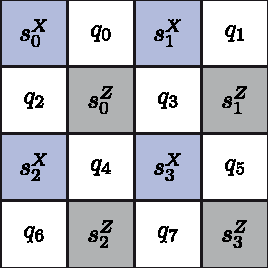
\includegraphics[width=5cm]{assets/4-code.pdf}
  \end{center}
  \caption{Qubit lattice for the $4$-code. $s_{k}^X$ and $s_{k}^Z$ are $X$- and $Z$-stabilisers represented by the sites respectively. $q_i$ are qubits. By way of example, $s_{0}^X = X_0 X_2 X_1 X_6$ and $s_{0}^Z = Z_3 Z_4 Z_2 Z_0$.}
  \label{4-code}
\end{figure}

We let $S_X = \{s^X_{k}\}$. There are $n^2$ elements in $S_X$, but only $n^2-1$ independent elements, as the final element is the product of all the others. We similarly define $S_Z = \{s^Z_{k}\}$. We will later use the sets $S_X$ and $S_Z$ to define the stabilisers of the codespace. Practically we will make measurements of these operators to check whether the state is still in the codespace. 

Just as in Shor's code, to fully define a state we will need to add additional independent, commuting operators to our set of stabilisers. We now construct a set of operators that will be used for this purpose. We define $X_h$ (horizontal X) to be the product of $X_i$s acting on qubits in an even row, $X_v$ (vertical X) the product of $X_i$s acting on qubits in an even column, and similarly, $Z_h$ to be $Z_i$s on an odd row, and $Z_v$ to be $Z_i$s on an odd column. We will use the pairs, $\{X_v, Z_h\}$ and $\{X_h, Z_v\}$, to define the two logical qubits: each pair shares exactly one physical qubit and because of this it is possible to show that the operators anti-commute, as qubit operators should.  Any of the remaining pairs $\{X_v, X_h\}$, $\{X_v, Z_v\}$, $\{Z_v, Z_h\}$, and $\{Z_h, X_h\}$ can be used to initialise our two qubits, and suffice to fully define the state. We call this set the \textit{logical operators}, $L = \{X_v, X_h, Z_v , Z_h\}$, on our pair of independent \textit{logical qubits}. 

We will now turn to how errors are detected in the toric code. As with the treatment of the Shor code we will consider an error to be a set of individual $X$ and $Z$ errors applied to a subset of the physical qubits. An $X$-error on a single physical qubit will flip the eigenvalue of the neighbouring $Z$-stabilisers, but commutes with the $X$-stabilisers and will not be detected by them. This can be verified by checking the commutation relation of the operators for the stabiliser and physical error. We say that an $X$-error causes the neighbouring $Z$-stabiliser sites to \textit{fire}. Similarly, a $Z$ error will be detected by the $X$-stabilisers and not the $Z$-stabilisers, and a $Y$ will be detected by both sets. Additional errors will cause the stabiliser eigenvalues to toggle. If errors occur sequentially they will be detected by the stabilisers at either end of the chain (see Fig.~\ref{basic_errors}).

\begin{figure}[htb]
  \begin{center}
    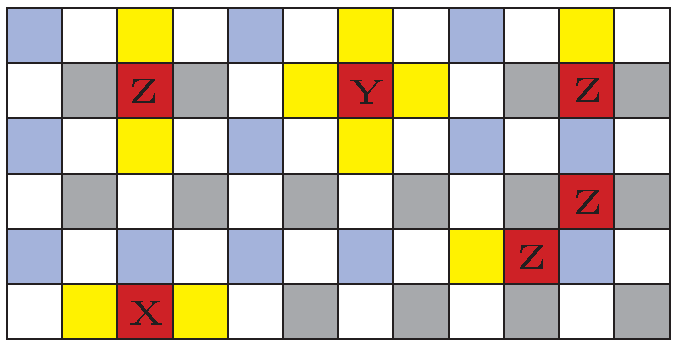
\includegraphics{assets/basic_errors.pdf}
  \end{center}
  \caption{Error detection of isolated $Z$-, $X$-, $Y-$errors and a chain of $Z$-errors. Error qubits are shown in red and firing stabilisers in yellow.}
  \label{basic_errors}
\end{figure}

\section{Code Variants}

In the rest of the chapter, we will consider three variants of the toric code, that we refer to as the \textit{classical toric code}, the \textit{reduced quantum toric code} and the \textit{full quantum toric code}.

\subsection{Classical Toric Code}

In the classical toric code we completely ignore the phase of each qubit, concerning ourselves only with the outcomes of measurements on the logical qubits in the $Z$-basis. To define the codespace we take our set of code stabilisers $S$ to be the set $S_Z$ and the set of logical operators $L=\{Z_h, Z_v\}$. We have the same geometry and number of physical qubits as described but only measure a reduced set of stabilisers. The codespace is massively degenerate but any state in it will be sufficient for our purposes.

We simplify the analysis by considering only $X_i$ errors on the individual qubits, as these are the only ones that can affect the measurement outcomes we are interested in. We define the complete set of error operators, $E$, to be the set generated by the individual physical qubit $X_i$ operators - that is the set of all products of such operators. As the $2n^2$ individual qubit operators, $X_i$, commute with one another and as $X_i^2 = \id$ we can show that $|E| = 2^{2n^2}$.

We also introduce the set of \textit{syndromes}, $A$ - the possible outcomes when the code stabilisers $S$ are measured. When each stabiliser measurement outcome is $+1$ we say we have obtained the \textit{zero-syndrome}, which we denote by the element $a_0 \in A$. If we obtain the zero-syndrome we know that we are in the codespace. In the classical toric code we have that $|A| = 2^{n^2-1}$, as each of the $n^2$ elements of $S$ can report $\pm 1$, but the last outcome is fixed by the others.

\subsection{Full Quantum Toric Code}

For the full quantum toric code, we aim to fully protect our encoded qubits against all sources of error. We take a full set of code stabilisers, $S = S_X \cup S_Z$, and the full set of logical operators $L = \{Z_h, Z_v, X_h, X_v\}$. The complete set of errors is generated by the set of all individual qubit operators $\{X_i, Z_i\}$, so that $|E| = 4^{2n^2}$.

Following similar reasoning to the classical toric code we can deduce the size of the set of syndromes, $A$: the outcomes of each of the $2n^2 - 2$ independent stabilisers in $S$ completely define a syndrome, so that $|A| = 2^{2n^2-2}$.

\subsection{Reduced Quantum Toric Code}

The reduced quantum toric code is slightly more subtle than the previous two cases. We take the full set of stabilisers $S = S_X \cup S_Z$ and logical operators $L = \{Z_h, Z_v, X_h, X_v\}$, but aim only to protect against individual qubit $Y_i$ errors. As previously, it is straightforward to show that $|E| = 2^{2n^2}$. It is more difficult to determine the size of $A$ in this case, as not all syndromes are possible from the errors that we consider. It is possible to show that $|A| = 2^{2n(n-1)}$ but this requires a deeper understanding of the structure of the code - which we will now develop.

\section{The Structure of the Code}

We now describe the structure of the set of errors, $E$, and how they relate to the syndromes, $A$, and logical errors, $L$. We take the definition of $E$ from the previous section: each `error' in $E$ is actually a set of Pauli operations of the physical qubits. We begin by defining the function
\begin{align}
  \text{synd}: E \rightarrow A
\end{align}
that maps an error onto its associated syndrome. We are then able to define
\begin{align}
  E_a = \{ e\in E : \text{synd}(e) = a \},
\end{align}
the set of all possible errors corresponding to a syndrome $a$. For convenience we define $E_0 = E_{a_0}$ to be the set of errors corresponding to the zero-syndrome, $a_0$. If an error in $E_0$ occurs it will go undetected by the code. This error has mapped a legitimate code state either onto itself or onto another legitimate code state; in the latter case inducing a logical error. We define a function to act on the set $E_0$,
\begin{align}
  \text{lerr}: E_0 \rightarrow L,
\end{align}
taking an error to the corresponding logical error on the encoded qubits. The possible logical errors on the logical qubits are precisely the same as the logical operators $L$ that we defined earlier. Finally we define the set
\begin{align}
  E_{0, l} = \{ e\in E_0: \text{lerr}(e) = l \}.
\end{align}
It is easy to see that each $E_{0, l}$ contains at least one element, as $l$ itself is a member: Our code contains the ability to perform logical operations on our code state. These operations could happen in an error sequence and so $l \in E_{0,l}$. We will now show that the sets $E_{0,l}$ have exactly the same number of elements - our first important observation about the structure of our toric codes. It may be useful to refer to Fig.~\ref{e_0}, which provides a graphical representation of the result for the classic code, whilst reading the section.

\begin{figure}[htb]
  \begin{center}
    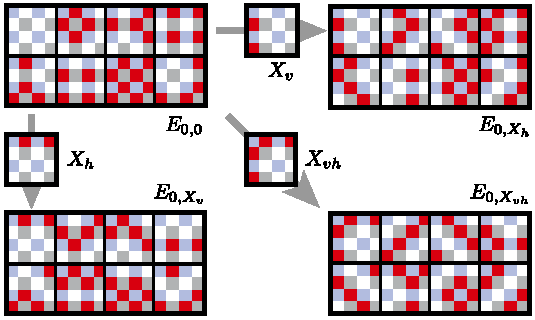
\includegraphics{figures/e_0.pdf}
  \end{center}
  \caption{$E_0$ for the classic toric code. The red squares represent physical $Z$-errors. The set $E_{0,0}$ combined with the logical errors $\{X_v, X_h, X_{vh}\}$ generate the $E_{0, l}$.}
  \label{e_0}
\end{figure}

To show that the $E_{0, l}$ are all the same size, we will show that they all have the same number of elements as $E_{0,0}$ - the set of elements of $E_0$ that introduce no logical error. To see this, take element $e_1 \in E_{0, l}$ and $e_2 \in E_0$. We claim that
\begin{align}
  e_2 \in E_{0, l} \Leftrightarrow e_1 e_2 \in E_{0,0}, \qquad \forall e_1 \in E_{0,l}.
\end{align}
The proof of the claim follows from the fact that all logical operators $l\in L$ are products of individual qubit operators, so that $l^2 = \id$: by applying the same logical error twice we undo it. If by applying $e_1$ after $e_2$ we have no logical error, they must be in the same error class, and the converse is also true. We now consider the set
\begin{align}
  e_1 E_{0,0} = \{e_1 e : e \in E_{0,0}\}
\end{align}
and claim that, given $e_1 \in E_{0,l}$, we must have $E_{0, l} = e_1 E_{0,0}$. This follows as, 
\begin{align}
  e_2 =  e_1 e \Leftrightarrow e_1 e_2 = e,
\end{align}
where we have used that $e_1^2 = \id$. Therefore we can use $e_1$ to establish a bijection between $E_{0,l}$ and $E_{0,0}$ and so the sets must have the same number of elements.

We now move on to the sets of errors, $E_a$, corresponding to a general syndrome, $a \in A$. As we have taken $A$ to be the set of obtainable syndromes, it follows that there must be at least one element in each set $E_a$. It is useful to assume that we have chosen an arbitrary member from $E_a$. We call this a \textit{matching} for the syndrome, and denote our specific choice of matching $m^*(a)$. In practice there are many ways to construct a specific matching for each syndrome $a$, for example see Fig.~\ref{matching}. If we observe the syndrome $a$ and apply the matching $m^*(a)$ we are guaranteed to be back in the codespace.

\begin{figure}[htb]
  \begin{center}
    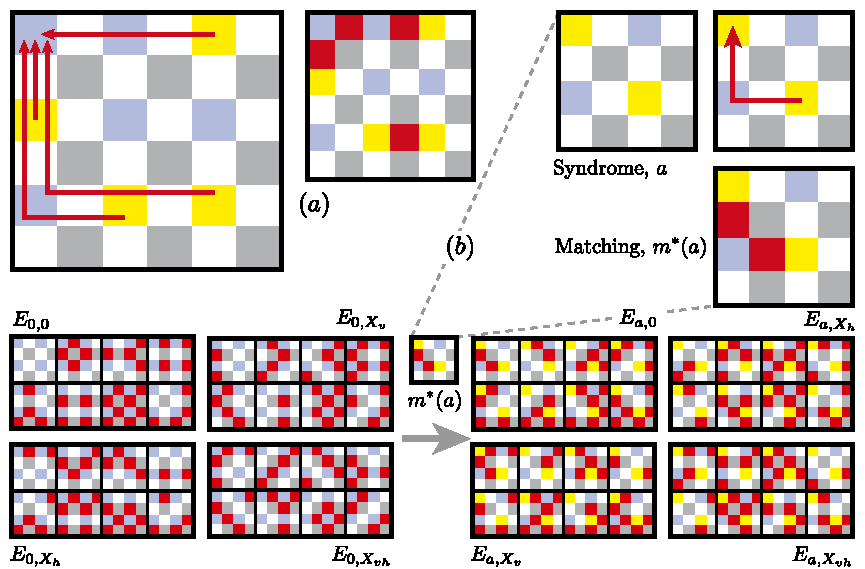
\includegraphics{figures/e_a.pdf}
  \end{center}
  \caption{Part (a) shows the method we use for constructing a matching from a syndrome: all firing stabilisers are `pushed' to the left, then to the top. A $Z$-operation is performed on any qubit that has been passed over an odd number of times. Part (b) shows how to use a matching $m^*(a)$ for a syndrome $a$ to generate the set $E_a$ from the set $E_0$.}
  \label{matching}
\end{figure}

Following a similar procedure to before we can show that $E_a = m^*(a) E_0$, and therefore each of the sets $E_a$ have the same number of elements. Furthermore we can split the set $E_a$ up into a set of classes
\begin{align}
  E_{a,l} = m^*(a) E_{0, l}.
\end{align}
The set $E_{a,l}$ can be interpreted as the set of errors that when corrected by $m^*(a)$ induce the logical error $l$ on the encoded qubits. All the sets $E_{a, l}$ have the same number of elements as $E_{0,0}$.

\begin{figure}[htb]
  \begin{center}
    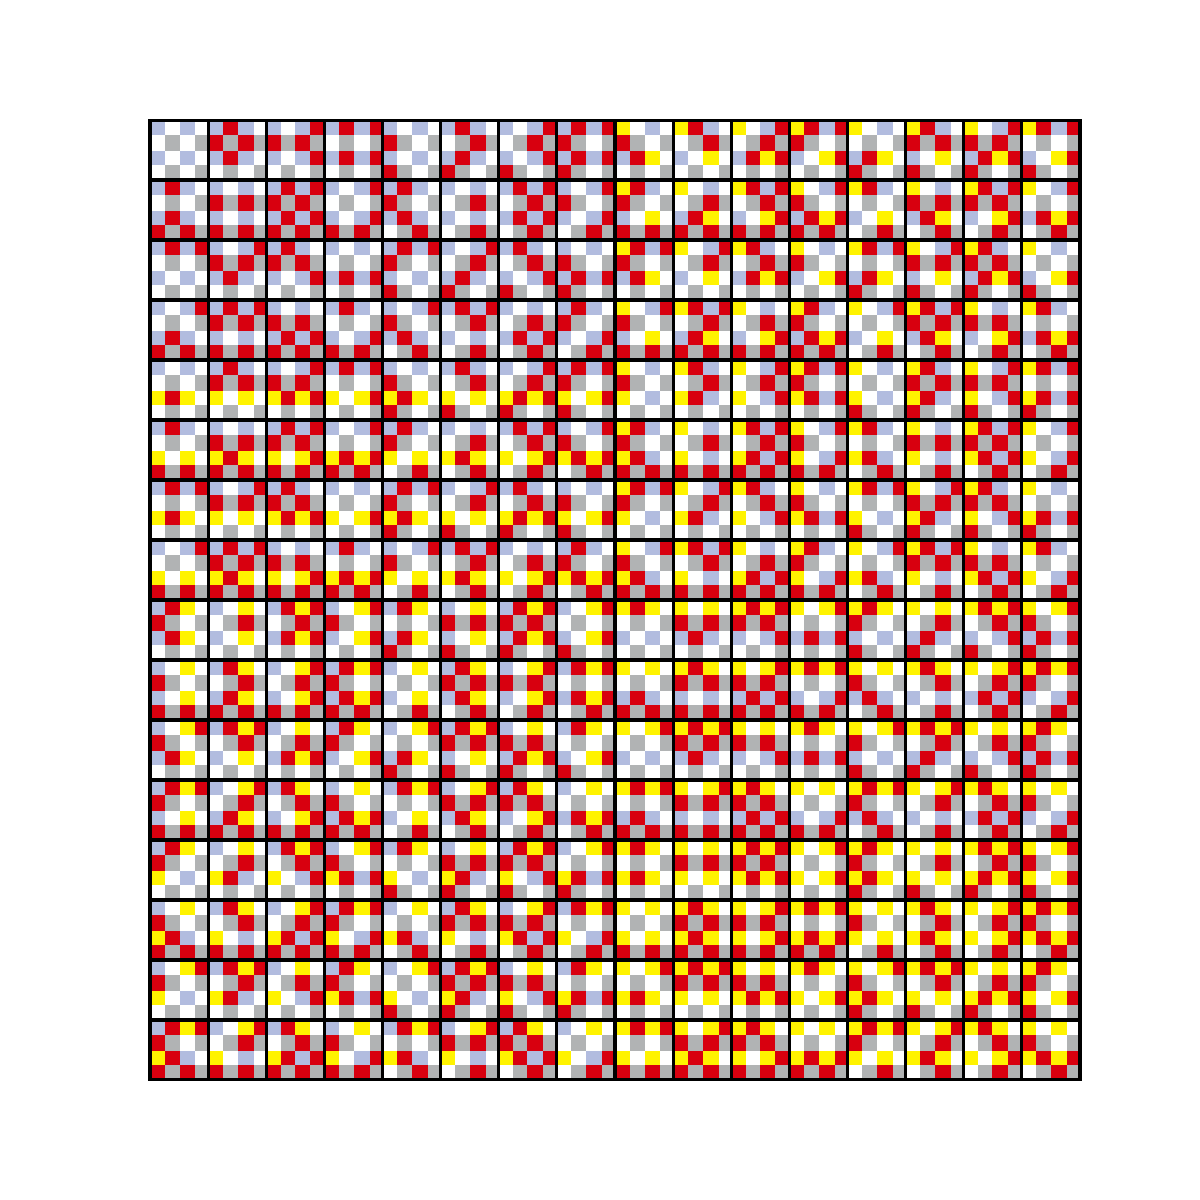
\includegraphics{figures/4_array.pdf}
  \end{center}
  \caption{Full set of errors, $E$, for the classical $4$-code. $E_{0,0}$ and $E_0$ have been separated from the rest to highlight their role in generating the complete set $E$.}
  \label{4_array}
\end{figure}

In the preceding paragraphs we have split up the total set of errors $E$ into identically sized subsets $E_{a, l}$ indexed by $a\in A$ and $l\in L$ (Fig.~\ref{4_array}). It follows immediately that
\begin{align}
  |E| = |A| \cdot |L| \cdot |E_{0,0}|.
\end{align}
One can see that this relationship holds for our three code variations in Table~\ref{code_sizes}.

\begin{table}
  \begin{center}
    \begin{tabular}{c c c c c}
      Code & $|E|$ & $|A|$ & $|L|$ & $E_{0,0}$ \\[1.5ex]
      \hline \\[0ex]
      Classical         & $2^{2n^2}$ & $2^{n^2-2}$ &  4 & $2^{n^2-2}$ \\[3ex]
      Reduced Quantum   & $2^{2n^2}$ & $2^{2n(n-1)}$ &  4 & $2^{2n-2}$ \\[3ex] 
      Full Quantum      & $4^{2n^2}$ & $2^{2n^2-2}$ & 16 & $2^{2n^2-2}$
    \end{tabular}
  \end{center}
  \caption{Sizes of the sets involved with our three toric code variants.}
  \label{code_sizes}
\end{table}

We have shown that given a syndrome always corresponds to multiple logical error classes, of which we can correct only one. We still have to answer the question of which one to correct. In the Shor code case we picked the matching to minimise the probability of introducing a logical error. Ideally that is what we would do here too. This of course depends on the error model, which we have not discussed yet. It is also not straightforward to do. The number of matchings in each class grows exponentially with the size of the grid. No efficient way of calculating the probabilities is known, even for the simplest error model.

The job of picking a matching given a syndrome falls to a decoder. These are often heuristic procedures, designed to balance calculation time with identifying the most likely class as often as possible. Determining a good decoding strategy is currently a very active area of research and there are a number of different approaches \cite{poulin_renormalisation, fowler_classical_processing, wooton_mcmc1}. It is not only important that a decoder maximises the probability of returning to the codespace without inducing an error on the logical qubits, but also that the decoder can run in a reasonable amount of time. 


%\subsection{Existing Decoding Strategies}

%Determining a good decoding strategy is currently a very active area of research. It is not only important that a decoder maximises the probability of returning to the codespace without inducing an error on the logical qubits, but also that the decoder can run in a reasonable amount of time. Here we look at three leading decoding strategies: minimum weight path matching, renormalisation, and Markov chain Monte Carlo.

%Minimum weight path matching (MWPM) aims to minimise a cost associated with the matching. The first stage of the algorithm is to take the firing stabiliser sites and place them on the nodes of a graph. An edge is then constructed between each pair of nodes with a weight representing the cost of connecting the sites on the lattice. A common choice is to take the Manhatten distance between the nodes, but it is possible to construct different weights to take addition information into account such as inhomogeneous error rates. Edmond's minimum weight path matching algorithm is then run on the graph, to pair up all the nodes whilst minimising the total weight of the edges chosen. This procedure is run separately on the $X$- and $Z$-syndromes, but it is possible to modify the procedure to take into account correlations between the syndromes caused by $Y$ errors.

%MWPM is $O(n^2)$ in the length of the lattice \cite{fowler11}. It provides good results especially in the low error case, when the minimum weight matching has a high probability of belonging to the most likely error class. Conceptually it is a little unsatisfactory that the algorithm is not truly aiming to find the most likely error class. The other two strategies have been shown to outperform MWPM in the case of high error rates, but this point is somewhat moot as it is unlikely that a quantum computer would function in this regime. A more troubling feature is that there is no natural way to incorporate additional classical information that may be available from the experimental procedure beyond altering the edge weights in an ad.\ hoc.\ fashion.

%The renormalisation approach involves splitting the lattice into sublattices, producing a matching on the sublattices and then combining the results to produce a matching for the complete lattice. The approach is recursive, in that the same procedure is applied to each sublattice. 

%The Markov chain Monte Carlo method aims to estimate the probabilities of each of the error classes consistent with the observed syndromes, by randomly sampling from each class using the Manhatten algorithm. 


\section{Error Model}

We consider depolarising noise distributed uniformly over the lattice with a given, constant probability:
\begin{equation} \label{noise_eq}
  D(\rho) = p_x X\rho X +  p_z Z\rho Z + p_y Y\rho Y  + (1- p_x - p_y - p_z)\rho.
\end{equation}
The values of $p_x$, $p_y$ and $p_z$ vary over our different code variants accordingly
\begin{enumerate}
  \item Classical case: $p_x = p$, $p_y = p_z = 0$
  \item Reduced quantum case: $p_y = p$, $p_x = p_z = 0$
  \item Full quantum case: $p_x = p_y = p_z = p/3$.
\end{enumerate}

We also consider the effect of stabiliser sites mis-reporting the stabiliser measurement outcomes: that with some probability, $q$, the stabiliser outcome is reported as a $+1$ when it was $-1$, or a $-1$ when it was $+1$.

In the literature, faulty stabiliser evaluations are often dealt with by extending the code into a third dimension. This treats the case when multiple rounds of faulty stabiliser evaluations are performed, where there is benefit to considering the history of the stabiliser outcomes as well as the current value. Here we consider only one round of stabiliser evaluations, so instead aim to identify and correct the most likely true stabiliser result given the outcome we observed. Even in the multiple evaluation round case, the last stage would involve a procedure similar to ours, so our results provide an upper bound on the decoding probability: you would not use this approach on each stage of a multi-round scheme, but those previous rounds certainly will not increase your probability of a successful decode in the last step.

\section{A Precomputed Decoder}

We begin by looking at the probability of getting a particular logical error, $l$, given that syndrome, $a$, occurs and we attempt to correct it using our chosen matching method by applying $m^*(a)$:
\begin{align}
  p(l \vert a) = \sum_{e \in E_{a,l}} \frac{p(e)}{p(a)}. 
\end{align}
For each stabiliser outcome $a$ we identify the most likely logical error $l_a$, such that $p(l_a \vert a)$ obtains a maximum\footnote{In cases where the most likely logical error is not unique we pick arbitrarily between the candidates.}. We may then correct our earlier attempt by applying the operator $l_a$, so that the total correction operation on the state will be $l_am^*(a)$. The overall successful decoding probability from following this procedure is 
\begin{align}
  P_d &= \sum_{a \in A} p(l_a \vert a)p(a) \\
  &= \sum_{a \in A} \max_{l\in L} \left\{ \sum_{e \in E_{a,l}} \frac{p(e)}{p(a)} \right\} p(a) \\
  &= \sum_{a \in A} \max_{l\in L} \left\{ \sum_{e \in E_{a,l}} p(e) \right\}. \label{truthful_prob}
\end{align}

When considering mis-reported stabiliser outcomes we can no longer assume that the syndrome we observe will be in $A$. We let $A'$ be the set of all possible stabiliser outcomes $A' = \{0, 1\}^{\otimes n^2}$. If we are to successfully decode a syndrome $a'$, we must first identify the correct syndrome $a$, on which to perform the arbitrary matching, and then identify the most likely logical error $l_a$ to correct. If we identify the wrong $a$, the final state will not even be in the code space. Given $a'$ we must pick $a$ and $l$ to provide the maximum probability of a successful decoding in the case of mis-reporting stabiliser outcomes:
\begin{align}
  P'_d &= \sum_{a' \in A'} p(\text{success} \vert a') p(a') \\
  &= \sum_{a'\in A'} \max_{a \in A} \left\{ p(l_a \vert a) p(a \vert a') \right\} p(a')\\
  &= \sum_{a'\in A'} \max_{a \in A} \left\{ \max_{l \in L} \left\{\sum_{e \in E_{a,l}} \frac{p(e)}{p(a)} \right\} p(a \cap a') \right\}\\
  &= \sum_{a'\in A'} \max_{a \in A} \left\{ \max_{l \in L} \left\{\sum_{e \in E_{a,l}} p(e) \right\} p(a' \vert a) \right\}. \label{lying_prob}
\end{align}
While equations (\ref{truthful_prob}) and (\ref{lying_prob}) are conceptually simple, calculations are beset by difficulties due to the rapid growth in the size of the sets $E_{a,l}$, $A$, and $A'$: in the single noise channel case for the $2n$-code $|E_{a,l}| = |A| = 2^{n^2-1}$; for the full noise channel $2n$-code $|E_{a,l}| = |A| = 2^{2n^2 - 2}$. For example, the total number of error configurations, $|E|$, for the $6$-code is $2^{36}$, which would require $\sim200$GB of storage space.

Thankfully, we do not need the complete set of error configurations to compute the value of $p_\text{success}$ in Eq.~(\ref{truthful_prob}). For each configuration $e\in E$ the probability is
\begin{align}
  p(e) = (1-p)^{2n^2 - n(e)} p^{n(e)}
\end{align}
where $n(e)$ counts the number of errors in error configuration $e \in E$. When summing over the errors consistent with a given logical error and syndrome we get
\begin{align}
  \sum_{e \in E_{a,l}} p(e) &= \sum_{e \in E_{a,l}} (1-p)^{2n^2 - n(e)} p^{n(e)} \\
  &= (1-p)^{n^2} \sum_{i = 0}^{2n^2} d_{a,l}^{(i)} \left(\frac{p}{1-p}\right)^i \\
  &=: (1-p)^{n^2} \chi_{a,l}\left(\frac{p}{1-p}\right)
\end{align}
where $d_{a,l}^{(i)} = \vert \left\{e \in E_{a,l} : n(e)=i \right\} \vert$ and we have used the final line to define the characteristic function $\chi_{a,l}$ of the class $E_{a,l}$. By computing and storing the coefficients $d_{a,l}$ we are able to calculate the success probabilities for a range of values of $p$.

The full source code used for our calculations, along with the computed tables of characteristic function coefficients, is available online \cite{toric_code_program}.

\section{Simulation Results}

\subsection{Classical Toric Code}

Using the method described, we calculated the success probabilities $P_d(n, p)$, and compared them with $p_{\text{bare}} = (1-p)^2$, the probability that two non-encoded qubits would remain error-free (Fig. \ref{x_results}).
\begin{figure}[htb]
  \begin{center}
    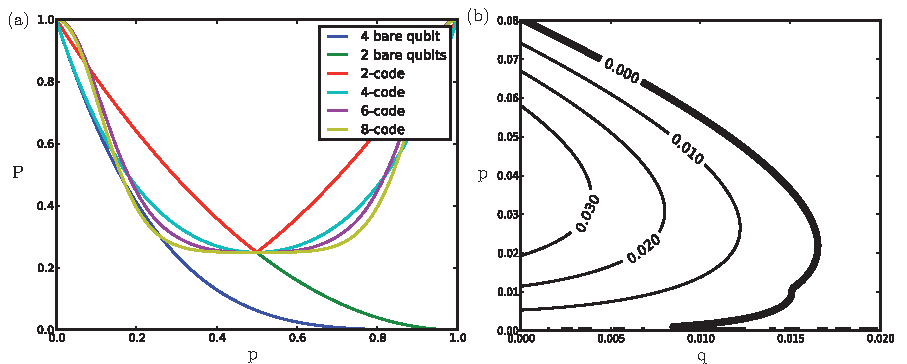
\includegraphics{figures/x_results.pdf}
  \end{center}
  \caption{Success probabilities for classical toric code: (a) shows the success probability, $P$, for ideal version of the code vs.\ the error rate, $p$, with two and four unprotected qubits for comparison; (b) shows the power of the $6$-code in the case when stabiliser outcomes are misreported with probability $q$.}
  \label{x_results}
\end{figure}

The $2$-code performs exactly the same as the bare qubits. This is not surprising, as the $2$-code has 2 physical code qubits and no error detect capacity - there is only one possible syndrome. For this reason, in future plots we omit $p_\text{bare}$, instead performing the comparison with the $2$-code. The $4$-code performs worse than the bare qubits. Although the $4$-code has error-detect capacity, it has no error correct capacity. This can be seen by considering the case when a single error occurs - due to the translational symmetry of the lattice, the syndrome can give us no information about whether our correction introduced a logical error or not. For the $4$-code to be successful there must be no errors on the $4$ qubits that $X_h$ and $X_v$ measure, an event with probability approximately equal to $(1-p)^4$ for small $p$.

The $6$-code is the smallest code that exhibits encoding power for some values of $p$. Provided that $p < 0.08$ the $6$-code outperforms the bare qubits. The $8$-code appears to offer roughly the same performance as the $6$-code. We were not  able to go beyond $2n=8$ with the computing resources available, but we expect that as $n$ increases the curves would tend towards a step function at the one-channel threshold.  We looked at the mis-reported stabiliser outcome case for the $6$-code. There is a small region with positive encoding power, that requires stabiliser fidelity in the region of $1\%$.

\subsection{Reduced Quantum Code}

For the reduced quantum code, we find that the $4$-code is the first code to offer encoding power in this scenario (Fig. \ref{y_results}). As before the $2$-code has no error detect capacity. Unlike before, the $4$-code is able to detect and correct errors, as it can use both $X$- and $Z$-stabiliser information to break the symmetry and pinpoint the error. 

We investigated the case of mis-reported stabiliser measurement outcomes for the $4$-code. We obtain positive encoding power for mis-reporting rates of up to 10\%. Overall the reduced quantum code shows remarkable encoding power, even for small codes. In using the full stabiliser information to detect a reduced set of errors, we have managed to hugely reduce the size of each error class (Fig.~\ref{code_sizes}). 
\begin{figure}[htb]
  \begin{center}
    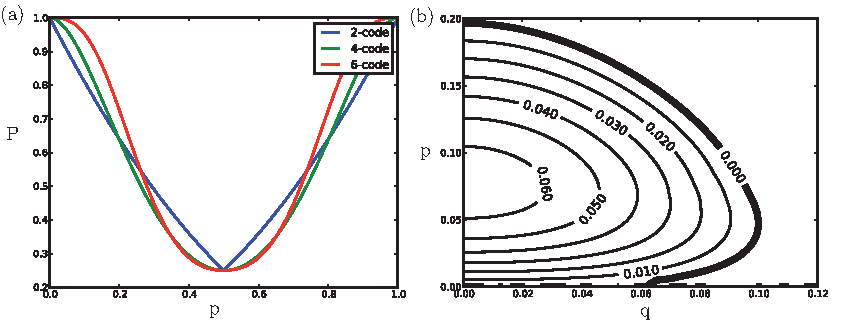
\includegraphics{assets/y_results.pdf}
  \end{center}
  \caption{Success probabilities for reduced quantum toric code: (a) shows the success probability, $P$, for ideal version of the code vs.\ the error rate, $p$, with two and four unprotected qubits for comparison; (b) shows the power of the $4$-code in the case when stabiliser outcomes are misreported with probability $q$.}
  \label{y_results}
\end{figure}

The circumstances that could justify the assumptions of the reduced quantum code are not unrealistic: we envisage a system with a single dominant error channel. In picking this to be the $Y$ channel, we exploit the lack of symmetry in our code effectively tailoring our code to be effective against the dominant error channel.

\subsection{Full Quantum Code}

Finally we look at the full code, protecting against full depolarizing noise, taking $p_x = p_y = p_z$ in equation (\ref{noise_eq}). 

\begin{figure}[htb]
  \begin{center}
    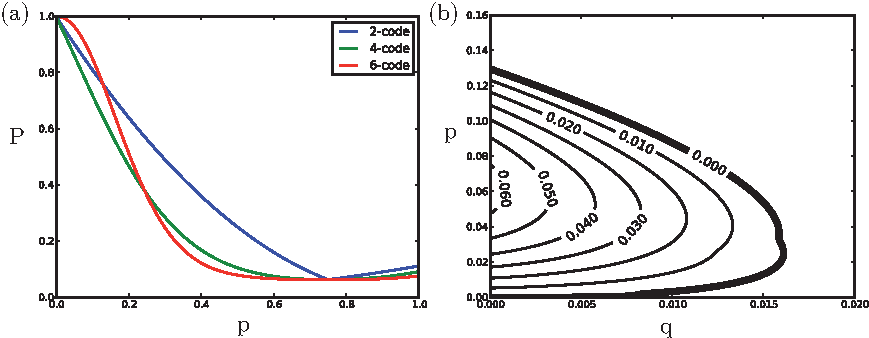
\includegraphics{assets/full_results.pdf}
  \end{center}
  \caption{Success probabilities for full quantum code: (a) shows the success probability, $P$, for ideal version of the code vs.\ the error rate, $p$, with two and four unprotected qubits for comparison. Note that the graph has a minimum at $p=0.75$ when the probability of each error is equal to the probability of no error. (b) shows the power of the $6$-code in the case when stabiliser outcomes are misreported with probability $q$.}
  \label{full_results}
\end{figure}

The $6$-code is the first code to offer encoding power (Fig. \ref{full_results}). We looked at mis-reported stabiliser outcomes for the $6$-code. Due to computational constraints we were only able to find a lower bound for $P'_d(p, q)$. This was obtained by modifying equation (\ref{lying_prob}) to maximise only over $a$ close to $a'$:
\begin{align} \label{approx_eq}
  P'_d= \sum_{a'\in A'} \max_{a \in N(a',x)} \left\{ \max_{l \in L} \left\{\sum_{e \in E_{a,l}} p(e) \right\} p(a' \vert a) \right\}
\end{align}
where $N(a', x) = \left\{a \in A : d(a', a) \leq x \right\}$ with $d(a', a)$ the number of stabilisers where $a'$ differs from $a$. We took $x = 2$ to produce a rough region, and then used $x=4$ to refine the boundary. 

\section{An Experimental Suggestion}

Our aim in this section is to provide a criterion which an experimentalist can use to verify whether a given candidate toric code set-up is providing protection.

Our criterion is based on the observation that the $2$-code is essentially equivalent to two unprotected qubits: the syndrome outcome is always $+1$ so we are unable to even detect errors and the logical operations reduce to single qubit operations. By comparing the performance of the candidate code system against that of the $2$-code we are able to say whether the candidate system is exhibiting protective power. 

We do not specify the decoder that the experimentalist must use for the larger code (decoding is trivial in the $2$-code), but our precomputed decoder will give optimal results. In our analysis we assumed that the stabiliser mis-reporting and physical qubit errors are independent events. A round of stabilisers is permitted to introduce physical qubit errors, but these must be sprinkled evenly over the lattice and not be correlated with mis-reporting sites. If strong correlations were to exist a modified decoder would give a better chance of satisfying the criterion.

We assume that an experimentalist has the ability to perform all $X$- and $Z$-stabiliser measurement operations and the logical measurements. In a large code the logical operations are potentially tricky, given their non-local nature. Here, due to the size of the codes considered, the logical operations actually involve fewer qubits than the stabilisers, and so are likely to be less technically demanding.

Our experimental proposal is as follows:
\begin{enumerate}
  \item Measure  $X_v$, $X_h$, and the stabilisers to find initial syndrome $a'_i$ and logical qubit states $(x^v_i, x^h_i).$\label{first_step}
  \item Wait. Manually introduce noise if required.
  \item Measure $X_v$, $X_h$, and the stabilisers to find final syndrome $a'_f$ and logical qubit states $(x^v_f, x^h_f)$.
  \item Decode the calculated syndrome, $a' = a'_i \text{\,XOR\,} a'_f$, to find matching $m$. \label{decode_step}
  \item Modify $(x^v_f, x^h_f)$ to reflect what the outcomes would have been if we had applied $m$ before measurement to find $(x^v_m, x^h_m)$.
  \item If $(x^v_i, x^h_i) = (x^v_m, x^h_m)$ count the round as a success; if not, count the round as a failure.\label{last_step}
  \item Repeat steps \ref{first_step} to \ref{last_step} many times to calculate an experimental successful decoding probability $P_\text{d}^\text{expt}$.
\end{enumerate}

The procedure is then repeated for initial measurements of $X_vZ_v$, $X_hZ_h$ and $Z_hZ_v$. We then repeat this procedure for the $2$-code and compare the results: if the larger system outperforms the $2$-code protection is provided. 


\section{Conclusion and Further Work}

We have provided a protocol and pre-computed decoder for demonstrating toric encoding size at minimal scale. The fewest qubits with which one could implement the $2n$-code is $2n^2+1$, and in that case the `extra' qubit must be capable of performing gate operations with all others. For the $4$-code this is a requirement of $9$ qubits and for the $6$-code the requirement is $19$ qubits. The error rates provided are not unrealistic for current experimental systems. 

As further work, a natural extension would be to apply the procedure described here to other surface codes. The smallest planar code can be constructed with fewer qubits than the smallest toric code, so could provide an easy experimental realisation of the class of surface codes. It is unclear whether the lower degree of symmetry in planar codes would improve the successful decoding probabilities that we calculate or not. 

We also believe that the reduced quantum case is particularly interesting and merits further investigation. The figures given in Table~\ref{code_sizes} show an imbalance between the sizes of $A$ and $E_{0,0}$ not present in the other codes, which seem to be the source of the codes high tolerance both to physical qubit errors and to mis-reported stabiliser outcomes. The structure of the code is also highly specialised, to an extent that it may be possible to calculate the characteristic functions for the classes $E_{a,l}$ without resorting to a full space search. This would allow far larger sizes of code to be investigated. The reduced quantum code model could also be experimentally appropriate for systems where one error channel is heavily dominant.


